\chapter{ALGORITHM FOR TREES}
\label{chap:dpp}

In this chapter, we propose a new algorithm for computing Betweennness Centrality specifically for trees. Consider a tree $T \equiv (V,E)$ such that $|V|=n$ and $|E|=n-1$.
To compute Betweenness Centrality for a tree, the Brandes' Algorithm by default takes $O(n^2)$ time.
We propose an algorithm with time complexity of $O(n)$.


\begin{figure}[htp]
\centering
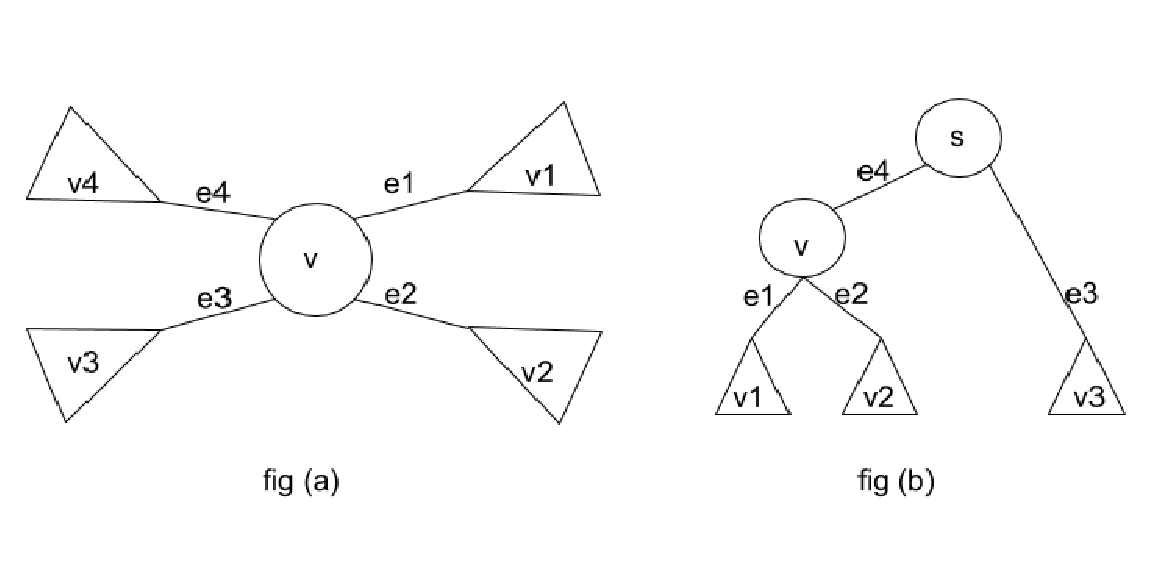
\includegraphics[width=13cm]{images/tree1.eps}
\caption{Reachable vertices of $v$}
\label{fig:lion}
\end{figure}

In figure \ref{fig:lion}(a) a vertex $v$ has four degree with edges as $e1,e2,e3,e4$ and $v1,v2,v3,v4$ corresponds to the number of vertices reachable through those edges respectively. We observed that any vertex from set $v1$ has a shortest path to any vertex in set $v2$ only through $v$. Same is applicable for $v1$ to $v3$, $v4$. Also other paths to be considered are from $v2$ to $v3, v4$ and $v3$ to $v4$.
So $bc[v] = v1*(v2+v3+v4) + v2*(v3*v4) + v3*v4$.

In general we can say that for a vertex $v$ with a degree $d$, $bc[v]$ can be calculated using the equation \ref{eq4} where $v_{i}$ corresponds to number of vertices reachable from $i_{}^{th}$ edge.

\begin{equation} \label{eq4}
bc[v] = \sum_{i=1}^{d-1} v_{i}*(v_{i+1}+..+v_{n})
\end{equation}

Hence for calculating betweenness centrality we need to determine the number of vertices reachable through each edge of that vertex.

The proposed algorithm is divided into two pass.
\vspace{-0.5em}
\begin{enumerate}

  \item Computes the number of reachable vertices for each edge of a vertex.
  \item Computes Betweenness Centrality for a vertex using the values computed in the first pass.
\end{enumerate}
\begin{algorithm}
\caption{Betweenness Centrality of tree}
Select a root vertex $s$ arbitrarily\;
pass1($s$,-1)\;
pass2()\;
\end{algorithm}


\hspace{-1.5em}The proposed algorithm is as follows:
\\
A vertex $s$ is chosen arbitrarily as root. First pass and second pass are then done on the tree considering $s$ as root.

\begin{figure}[htp]
\centering
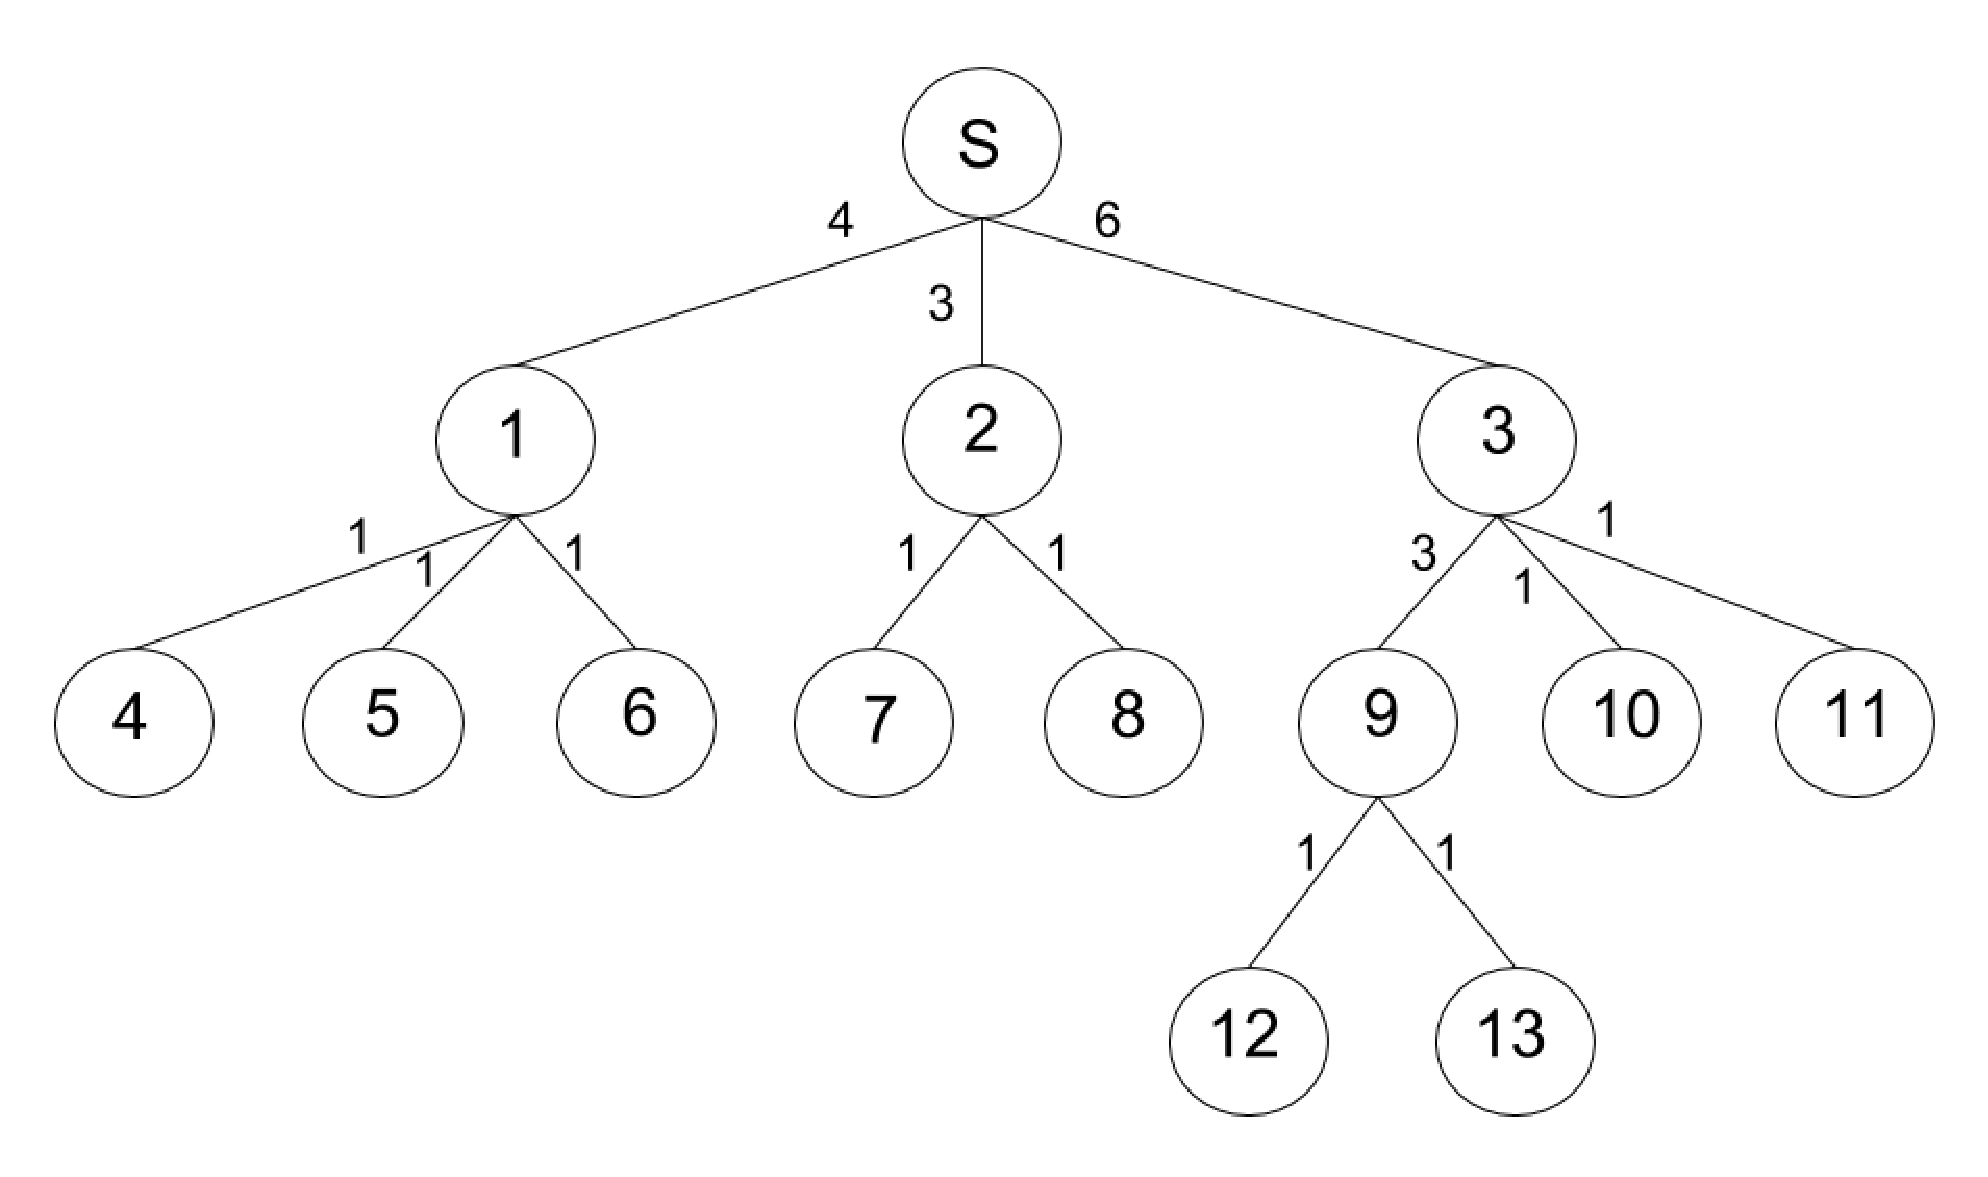
\includegraphics[width=13cm]{images/exampletree.eps}
\caption{Example of Tree}
\label{fig:extree}
\end{figure}

\section{First Pass of Tree Algorithm}
\begin{algorithm}
%\KwResult{Write here the result }
dfs$(child, parent)$ \\
$sum \leftarrow 0$\;

\For{each neighbour vertex $v$ of $child$}{
\If{$v \neq parent$}{
$temp \leftarrow$ dfs($v,child$)\;
$sum \leftarrow sum + temp$\;
Push $temp$ to list[$child$]\;
}
}
return $sum + 1$\;
\caption{Pass1 of Tree Algorithm}

\end{algorithm}
Depth First Search(DFS) is performed on tree starting from $s$. Every vertex $v$ returns the number of vertices in its own subtree including the vertex $v$ to its parent $p$. The parent vertex adds the returned value from all its children to its own list.
Vertex $v$ with a degree $d$ has a list of size $d$.
So at the at end of first pass, the list each vertex except source contains $d-1$ elements and source $s$ contains $d$ elements. The reason is that the source $s$ has no parent while every other vertex has exactly one parent. Hence, we need to add total number of vertices reachable through parent for all vertices except $s$.
For example, in figure \ref{fig:extree} vertex '9' returns a value 3 to its parent '3' and vertex 3 adds to its list. Similarly at the end of pass 1, vertex $S$ has values 4,3,6 in its list whereas vertex '3' has values 3,1,1. 
\vspace{-1.0em}
\section{Second Pass of Tree Algorithm}
\vspace{-1.0em}
So, in the second pass, the number of vertices reachable through parent $s$ of a vertex $v$ are determined.
In fig \ref{fig:lion}(b), we know values of $v1,v2$ but to calculate the number of vertices reachable from parent $s$ that is through edge $e4$, we can use the formula as
\\
no of vertices reachable through parent = total no of vertices - 1 - $(v1 + v2)$

In general we can say that,
\begin{equation} \label{eq5}
v_{d} = n - 1 + \sum_{i=1}^{d-1} list[v_{i}]
\end{equation}
where n is total number of vertices in graph, $v_{d}$ is number of reachable vertices through parent $s$.

For example, in figure \ref{fig:extree}, for vertex '3' its list contains values 3,1,1. So to calculate the number of reachable vertices through its parent, applying formula we get (14 - 1 - (3+1+1)) = 8 

After calculating $v_{d}$, it is added to $list[v]$.
Thus the calculated value 8 is added to list of vertex '3'.
Since we know the total no. of vertices reachable from all edges of a vertex, we can calculate Betweenness Centrality using the equation \ref{eq4}.
\\
Each pass visits each node once and thus the time complexity of the algorithm is $O(n)$.


\section{Proof Of Correctness}

For a tree, all the vertices are connected and have a single path and thus that path needs to be shortest. So the Betweenness Centrality value of a vertex $v$ becomes the total number of paths between any pair $s$ and $t$ passing through $v$, $s \neq t, v\neq t, s\neq v$. Now, such a $<s,t>$ pair whose shortest path passes through $v$, needs to be reachable from different edges of $v$. 

Let us assume that the betweenness centrality values calculated by our proposed algorithm is incorrect. Two cases arise that either our algorithm calculates more value of centrality or it calculates less than the actual value for a vertex $v$.

\begin{enumerate}
\item If our proposed algorithm has calculated more centrality value then for a pair $<s,t>$ whose shortest path does not contain $v$, some values are added to $bc[v]$. But according to Algorithm 2, it does not considers any pair $a,b$ which does not pass through $v$ and thus won't add any value to $bc[v]$.
\item If our proposed algorithm has calculated less centrality value then for a pair $<s,t>$ whose shortest path contains $v$, some values are not added to $bc[v]$. 
\\
Algorithm 2 considers does not considers the vertices reachable from same edge. Since pair $<s,t>$ is not considered, then it should be reachable from $v$ through same edge and thus contradicts the information that $v$ lies on shortest path from $s$ to $t$
\end{enumerate}

Thus, both this cases are not possible which proves that our proposed algorithm is sound and complete.